\chapter{Introduction}\label{ch:introduction}

\section{More crop per drop}
To feed a growing and wealthier population with changing dietary preferences, the Food and Agriculture Organization of the United Nations \parencite{fao2011} predicted that the world's annual agricultural production needs to increase by 70 \% between the year 2005 and 2050. Since less than 10\% of the required production increase can be achieved by expansion of arable land, the majority of the increase in food production will need to be realized by productivity gains. Such increases in crop productivity are to be attained either by increasing crop yields (77\%) or increasing cropping intensity (14\%).

Water scarcity is a major constraint for agriculture in many areas of the world. The International Water Management Institute (IWMI) estimated that one fifth of the world population lives in regions where the available water resources can not meet the water demand \parencite{molden2007a}. Aside from these 1.2 billion people facing physical water scarcity, another 1.6 billion of people live in areas with economical water scarcity. Although sufficient water is available in those areas, the water demand can not be met due to lack of infrastructure or financial resources. Currently, water demand for food production is one of the greatest pressures on freshwater resources. About 70\% of the world's fresh water is used by the agricultural sector \parencite{fao2014}. In some developing countries agriculture even accounts for up to 95\% of the total water withdrawl. In addition, agriculture competes with the increasing demand of water to sustain the ecosystem and meet the needs for human consumption, energy production and the industrial sector \parencite{fao2011}. 

Considering the widespread problem of water scarcity and the agricultural sector's insecure position of being a major water consumer, it is clear that availability of water will pose a serious constraint to increase crop productivity. For that reason, it will be crucial for the agricultural sector to increase not only crop yield but also crop water productivity, i.e. crop yield per unit of water consumed, in order to produce `more crop per drop'. 

\section{Upgrading crop water productivity in rainfed cropping systems}
Global statistics \parencite{fao2014} show that irrigated agriculture accounts for more than 40\% of global crop production on less than 20\% of the world's cultivated land. In spite of the high productivity of irrigated agriculture, a shift from rainfed to irrigated cropping systems is infeasible for many water-scarce regions in the world. Consequently, rainfed agriculture dominates world food production and will continue to do so in the future \textcite{fao2011}. Today, rainfed agriculture covers more than 80\% of the arable land and accounts for about 60\% of the global crop production. This dominance of rainfed agriculture is even stronger in water scarce regions of Sub-Saharan Africa where rainfed crops cover more than 95\% of the cultivated land \parencite{fao2014}. In addition, more  than  half  of  global  population  growth  between  now  and  2050  is  expected  to  occur  in  Africa \parencite{un2015}, where people still predominantly rely on rainfed crop production \parencite{fao2014}. 

Although high yield levels are attained in rainfed cropping systems of temperate regions with reliable rainfall and productive soils, the overall productivity of rainfed agriculture is low. Rainfed cereal yields range between 0.5 and \SI{2}{t/ha}, with an average of \SI{1}{t/ha} in Sub-Saharan Africa. \textcite{rockstrom2007c} report that these yields are 2 to 4 times below the achievable yield levels for major rainfed grain crops. In addition, rainfed yields are 2.7 times lower than those obtained in irrigated cropping systems \parencite{un2012}. \textcite{rosegrant2002} report that in developing countries cereal yield is on average \SI{1.5}{t/ha} for rainfed cropping systems, which is less than half of the average irrigated cereal yield of \SI{3.1}{t/ha}. Furthermore, \textcite{zwart2010} who simulated crop water productivity levels for wheat found that highest water productivity levels (up to 1.8 harvestable product per \si{m^3} of water evapotranspired) are obtained in temperate regions with high precipitation, whereas values between 0.4 and \SI{0.8}{kg/m^3} are more common in rainfed systems with low precipitation rates. Also \textcite{liu2007} report that low water productivity levels are more often encountered for rainfed cropping systems than for irrigated cropping systems. Due to these low productivity levels in rainfed agriculture, there is huge potential for upgrading crop water productivity, especially in low-yielding small-scale rainfed cropping systems in drought-prone regions \parencite{rockstrom2007c,molden2010}. 

Crop water productivity can be improved by developing drought-tolerant, disease-resistant or high-yielding crop varieties either via genetic engineering or by traditional breeding \parencite{passioura2006,bennett2003}. However, improved crop varieties may only increase crop water productivity when cultivated under good agronomic conditions that are rarely encountered in farmers' fields. Moreover, developing improved crop varieties is a time-consuming process while the need for improving agricultural productivity is urgent. Furthermore, controversy regarding potential harmful effects of genetically modified crops hinder widespread adoption. Aside from the use of improved crops, also improved agronomy can upgrade crop water productivity. There is a wide variety of agricultural management practices available that either improve yield by reducing yield-limiting factors such as nutrient deficiencies or soil salinity, or that optimize the use of the available water water resources \parencite{passioura2006,ali2008}. 

Optimizing the use of available rainfall is crucial for rainfed agriculture. By analyzing water balances of farmers' fields of rainfed tropical cropping systems (\autoref{fig:ch1_Wabal}), \textcite{rockstrom2003c} found that only a small fraction of rainfall (15-30\%) contributes to crop production through crop transpiration. At least 70\% of the rainfall is lost trough unproductive water losses by soil evaporation (30-50\%), percolation to the groundwater (10-30\%) and surface runoff (10-25\%). Furthermore, rainfed agriculture is subjected to the intermittent and unpredictable character of rainfall. This is especially true for rainfed cropping systems in semi-arid and dry subhumid areas, where crop production is restricted more by variable rainfall, dry spells and droughts than by low total rainfall amounts \parencite{rockstrom2007c,wani2008a}. It is clear that there is great potential to increase crop water productivity in rainfed cropping systems by agricultural management practices that reduces unproductive water losses on the one hand, and deal with rainfall variability on the other hand. 

\begin{figure}[tbhp]
	\centering
		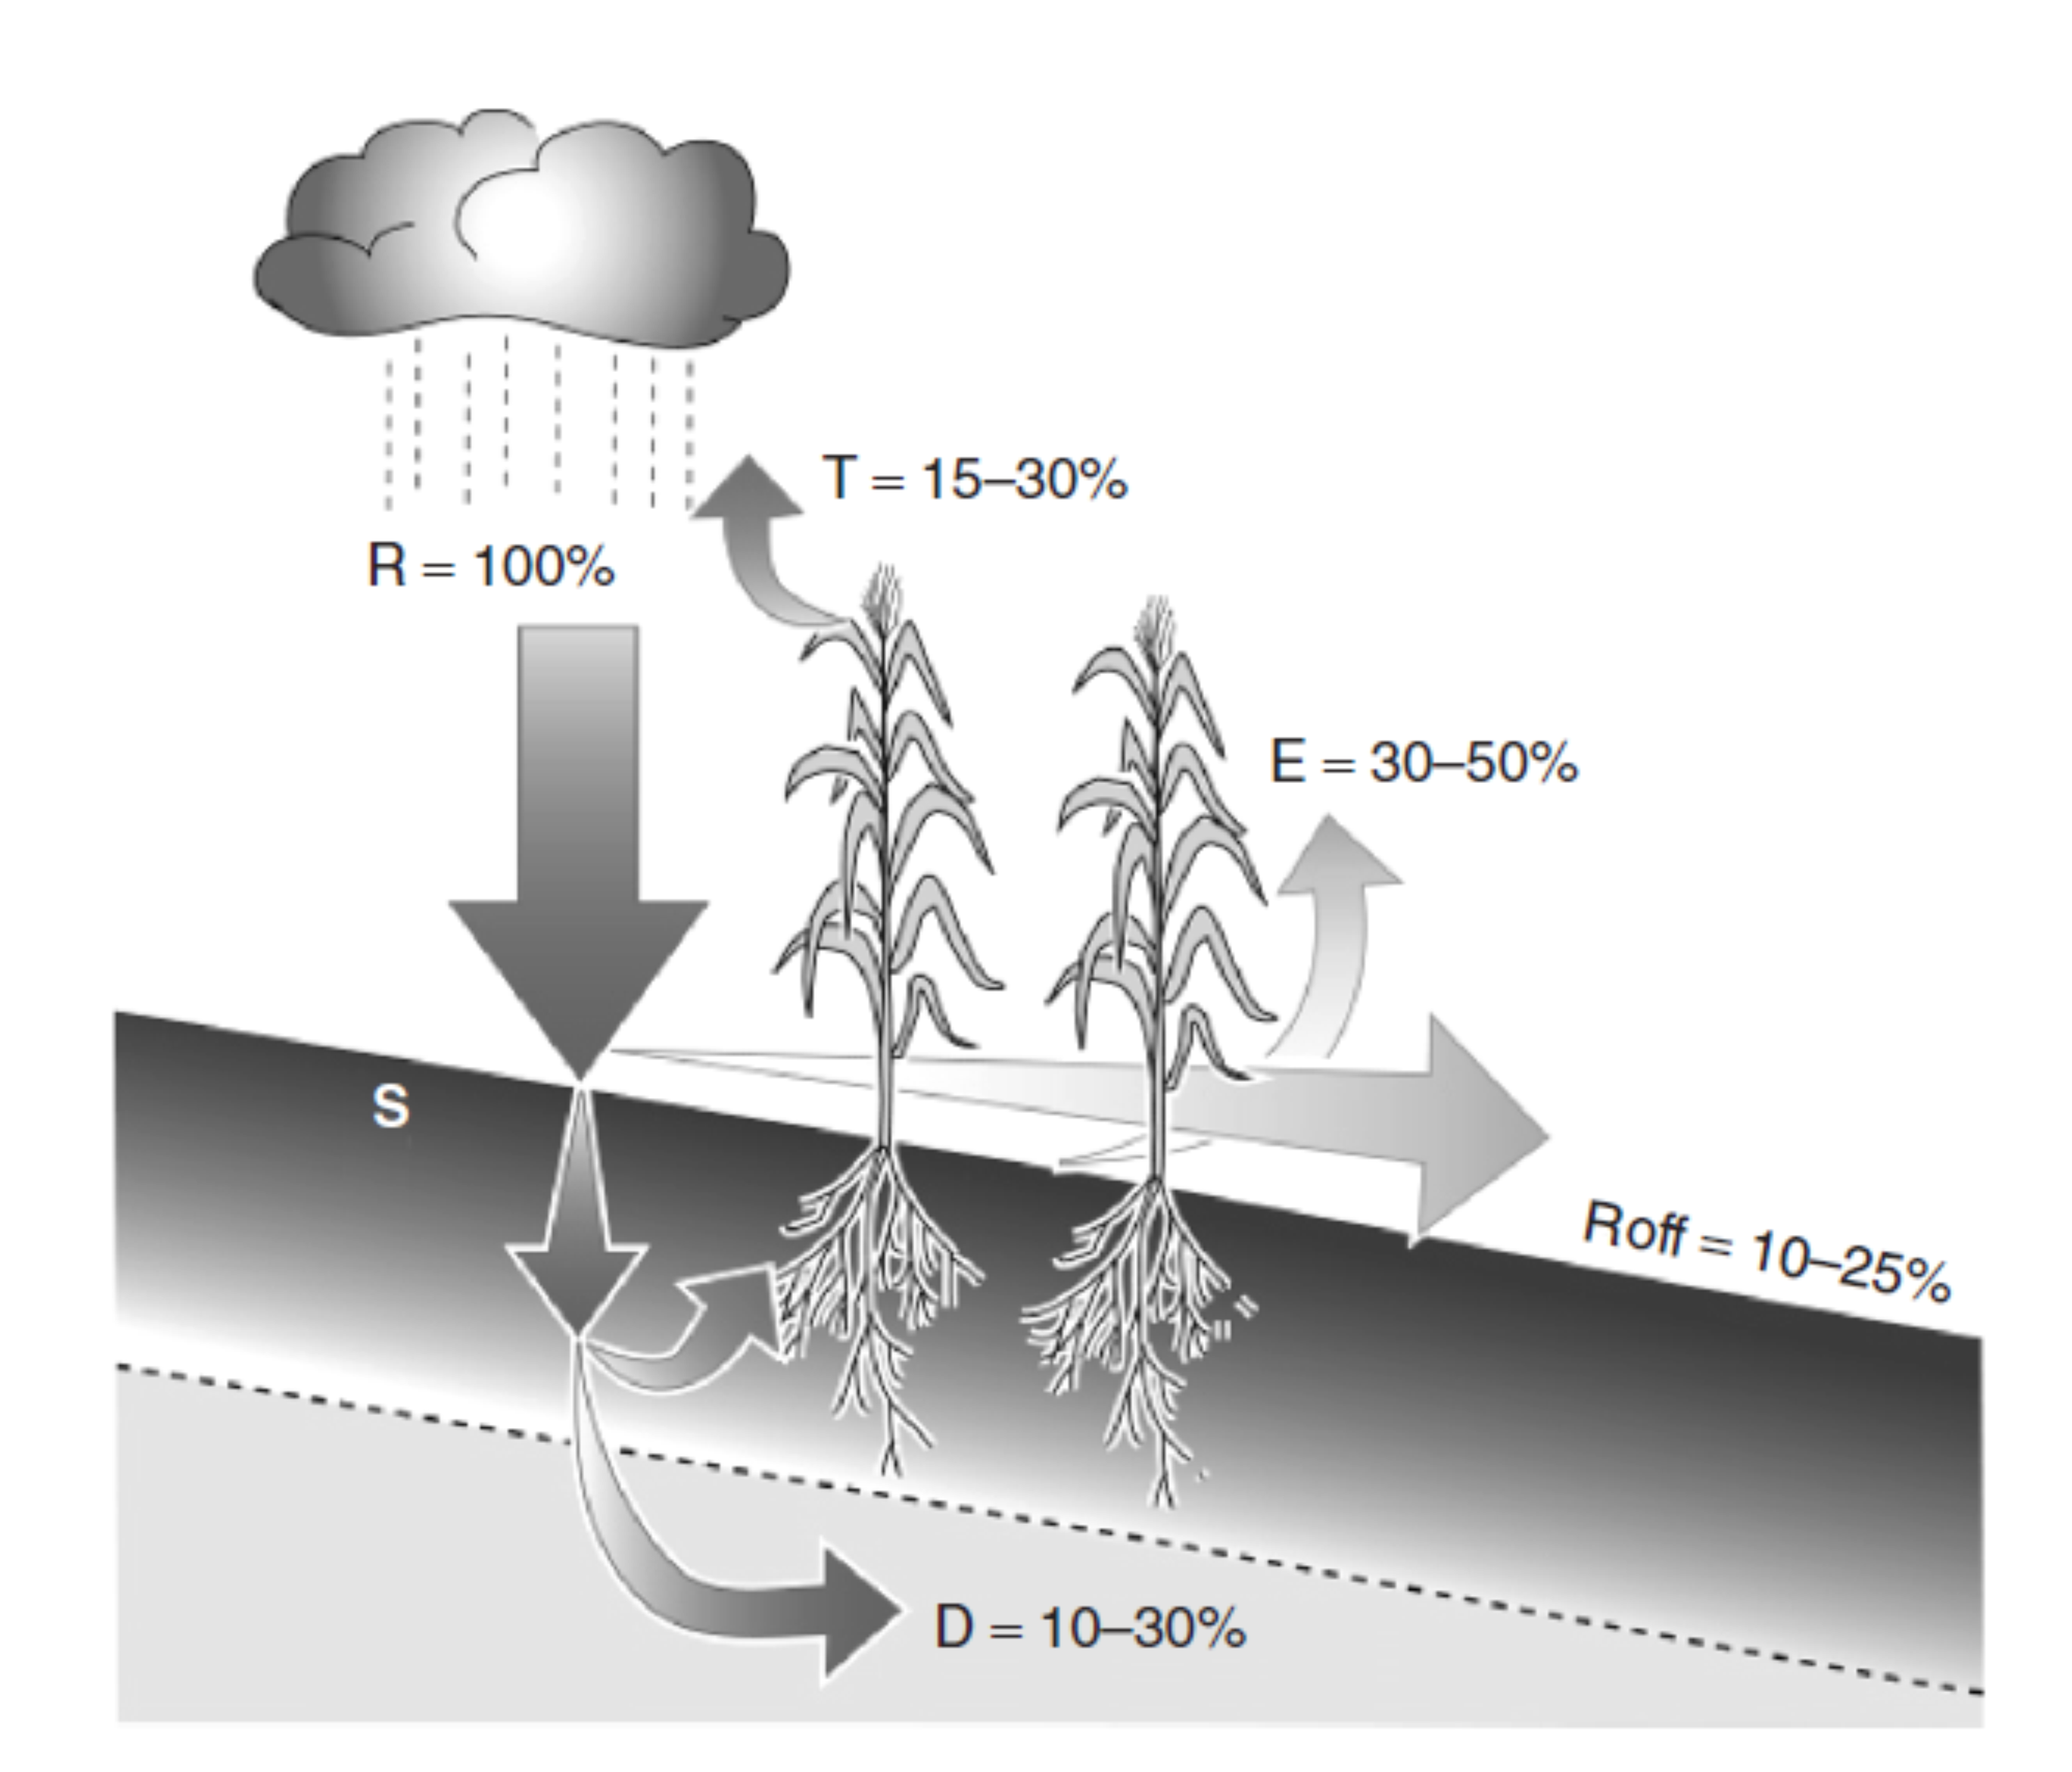
\includegraphics[width=8cm]{Wabal_600dpi.png}
	\caption{Rainfall partitioning in semi-arid tropical farming systems in Sub-Saharan Africa. S is soil moisture storage, R is rainfall, T is transpiration, E is evaporation, Roff is surface runoff and D is drainage (Source: \textcite{rockstrom2003c})}
	\label{fig:ch1_Wabal}
\end{figure}

Several studies have demonstrated the potential of various management strategies to increase crop yield and crop water productivity. \textcite{pretty2001}, who analysed 90 development projects on sustainable agriculture, concluded that intensification of a cropping system and optimizing the use of locally available natural resources could increase rainfed crop yields by 50\% to 100\% (with cases up to 700\% yield increase). Also efficient pest management shows great potential, since \textcite{oerke2006} found that global crop losses due to pests, including weeds, pest, pathogens and virusses, varied between 50\% and 80\% if no pest control practices are applied. Furthermore, with conservation agriculture, that focusses on minimal soil disturbance by no-inversion tillage, yield increases between 20 and 120\% were obtained in East Africa \parencite{wani2008a}. Integrated soil and fertility management that focuses on dry spell mitigation and soil fertility can potentially more than double yield in semi-arid rainfed farming systems while at the same time improve water productivity \parencite{rockstrom2007b}. In addition, a review by \textcite{hatfield2001} reports that soil management practices could increase crop water productivity by 25-40\%, while modifying soil nutrient management could increase water productivity by 15-25\%. 


\section{Agricultural production in a changing environment}	
Despite the large untapped potential in rainfed cropping systems, increasing food production in a sustainable manner requires more than optimizing crop water productivity for each individual farmer or field. Management practices that are beneficial for one farmer might negatively affect crop productivity in a neighbouring field, and consequently impede an overall growth of agricultural productivity. Therefore, researcher such as \textcite{molden2010,rockstrom2003c} stress the importance of water productivity analysis at basin scale, as upstream shifts in water partitioning might affect downstream water quality and quantity. In addition, the increase of crop productivity needs to take place in a rapidly changing world where population is growing, cities are expanding, productive land is getting scarce, several sectors and stakeholder struggle to get hold on the scarce natural resources (especially water) and society has to deal with the burden of environmental pollution and climate change.  

Climate change is projected to have a substantial impact on crop production and water availability. Increased atmospheric \COtwo concentration, altered rainfall patterns, higher air temperature, increased damage due to pest, diseases and weeds, and the increased incidence of extreme weather events under future climatic conditions will affect crop growth and production, as well as availability of important resources for crop production such as water and nutrients \parencite{ipcc2014}. Analysing more than 1090 projections, the Intergovernmental Panel on Climate Change \parencite{ipcc2014} found that the projected impact of climate change on crop production is highly variable, depending on the studied crop, region, adaptation scenario, emission scenario and time frame. For the near future (2030-2049), about 10\% of the projections indicate a yield increase of more than 10\% as compared to the late 20th century, whereas another 10\% of the projections show a yield loss of more than 25\%. After 2050, the risks of more severe yield loss increases. Generally, crop production will be negatively affected in low-latitude countries, while the impact might be postive or negative for northern-latitude countries. In addition, climate change is projected to increase inter-annual variability of crop yields in many regions. 

Also the projected effect of climate change on water availability has a high spatial variability, as changes in precipitation will not be uniform. Freshwater resources are projected to increase at high latitudes. By contrast, in most dry subtropical regions, climate change is projected to reduce renewable surface water and groundwater resources significantly. This will intensify competition for water among various sectors and consequently affect regional water, energy and food security \parencite{ipcc2014}.

Due to their effect on crop production and water availability, climate and other environmental changes will affect agricultural management, making some practices more or less effective than they are under current conditions. Also socio-economic factors might hinder adoption of certain agricultural management practices, even if they are very effective from an agronomic point of view. \textcite{molden2010} state that increasing water productivity is rarely a priority for farmers because they focus on increasing profitability or household food security. In addition, the interaction between agricultural production systems and their environment goes both ways. Changing agricultural management can also serve as a mitigation or adaptation strategy to counteract or deal with the adverse effect of environmental changes. The \textcite{ipcc2014} estimates that adaptation of agricultural management practices (including crop, irrigation and fertilizer management) could improve crop yield under future climatic conditions on average by about 15-18\% of the current yield levels as compared to a business-as-usual scenario. Seen the complex interaction of agricultural production systems with their environment, a sustainable increase of crop water productivity can only be achieved when both the on-site and off-site effect of agricultural management is evaluated, taking into account the interactions between crop water productivity, management and the changing environmental conditions. 

	
\section{Tools to evaluate agricultural management}	
Agro-hydrological models describe agricultural practices and hydrological processes, as well as their interactions, in cropped land areas. Therefore, they are suitable tools to investigate the impact of several agricultural management strategies under various environmental conditions on on-site crop water productivity as well as off-site hydrological processes \parencite{ferrant2014}.  

In contrast to empirical models that use observations to describe the relation between variables, physically-based models (also referred to as process-based or mechanistic models) describe the behaviour of a system based on established physical principles and laws. As a result, they have a high explanatory level and can be used to study processes transforming input into output variables. In spite of their process-based nature, also physically based models include some level of empirical generalization to fill physical knowledge gaps. This results in the need to calibrate those model against observations, although calibration requirements are lower than for empirical models. Conceptual models situate themselves in between empirical and physically based models, as they explain system behaviour based on empirical equations as well as preconceived notions on how the described system works. As both conceptual and physically based models allow representing dynamics of a system via simulation, they will be further referred to as simulation models \parencite{wainwright2004}. 

Nowadays, agro-hydrological simulation models are increasingly used because they enable efficient analysis of various scenarios on a wide spatial and temporal scale. That way they can be used to analyse policies and support strategic decisions on agricultural and water management. Moreover, simulation models allow investigation of interactions between various processes in the soil-plant-water-atmosphere continuum. In addition, model based research is mostly less expensive and time consuming than experimental research. Nevertheless, experimental data remain necessary for development, calibration and validation of the simulation models \parencite{wainwright2004}. 

Most agro-hydrological simulation models are characterized either as a crop model or hydrological model, even though evapotranspiration is an important and inseparable component of the hydrological cycle. 

Crop models focus on simulation of crop development and production. Typically, they operate at point scale (1D models) considering one homogeneous agricultural field. Due to the speed of crop development, crop models usually operate at a daily time step. Nowadays, more than 120 crop models are available \parencite{rivington2010}, each with their own strengths and weaknesses. These crop models differ with respect to the number and detail of processess that they incorporate, production situations they are dealing with (e.g. potential production versus actual production limited by various environmental factors), and their intended application domain and target audience (e.g. farmer advice tools versus research models to study resource use and efficiency)\parencite{holzworth2015,vanittersum2003,boote1996}.

Hydrological models describe hydrological processes within river catchments. These catchments, also referred to as river basins or watersheds, range in size from very small (e.g. the Plankbeek catchment in Belgium covers \SI{4.5}{km^2}) to several \SI{1000}{km^2} (e.g. the Amazon river basin covers \SI{7,050,000}{km^2}). Hydrological models represent a spatially heterogenous catchment either as a single unit (1D or dimensionless) with one set of characteristics and parameters (`lumped approach') or as a collection of several 2D or 3D units each with their own characteristics and parameters (`distributed approach'). Distributed models are further divided into `fully distributed' models such as MIKE-SHE \parencite{refsgaard1995}, and `semi-distributed' models such as SWAT \parencite{arnold1998a,douglasmankin2010}. The latter do not consider the spatial distribution of units within the catchment, while the former consider the exact spatial location of each unit and interactions between those units. Most hydrological models have a flexible time step for the simulation results that can be selected according to the catchment size and type of application. Flood modelling requires small time steps (hourly or even 15 minute time steps), whereas design of water storage structures can rely on simulations of water volumes at large time steps (daily, monthly or even yearly time steps).

Within the large collection of agro-hydrological simulation models, each model has its strengths but also limitations to investigate the effect of agricultural management on crop water productivity at field scale (on-site effect) and water availability at catchment scale (off-site effect). Since they operate at field scale, crop models have the disadvantage that they are not able to quantify the off-site effects of agricultural management. By contrast, distributed hydrological models are able to consider both field and catchment scale. However, as these models are primarily developed to study hydrological processes they have limitations for agronomic applications; Most hydrological models implement a restricted representation of crop development and transpiration, rarely simulate crop production and water productivity explicitly, and consider only few agricultural management practices affecting crop transpiration and production. The hydrological models that do include physically based equations to estimate crop transpiration and crop production as well as the effect of agricultural management, such as SWAT \parencite{arnold1998a,douglasmankin2010}, MIKE SHE \parencite{refsgaard1995} and APEX \parencite{gassman2010}, show relatively high computational complexity and data requirements. 

Despite the increasing possibility to use remote sensing data \parencite{boegh2004, moulin1998}, limited availability of data for input or calibration of agro-hydrological models remains a commonly encountered issue \parencite{grayson2002,boote1996}. Also hydrological models, especially the distributed ones, suffer from large data requirements \parencite{singh2006}. Conceptual models drastically reduce data requirements because of their simplicity. However, because of their conceptual nature model parameters can not be measured which again increases the need for calibration data. In the category of crop models, the AquaCrop model \parencite{hsiao2009,steduto2009,raes2009,vanuytrecht2014} is often cited as a model with low requirements for easily obtainable input data. Comparative studies by \textcite{abisaab2015, castanedavera2015,todorovic2009} note that this makes the model applicable in data-scarce regions. 

It is clear that a combination of several simulation models with low data requirements is needed to obtain a parsimonious simulation tool with full functionality to evaluate the on-and off-site agro-hydrological impact of agricultural management.

\section{Research objectives}
Given the limitations of existing agro-hydrological models to efficiently evaluate the potential of various agricultural management strategies to sustainably upgrade crop water productivity in an ever changing world, this PhD research intents to develop a new agro-hydrological model that
\begin{itemize}
\item simulates crop production and water productivity at field scale, as well as hydrological processes and water availability at catchment scale
\item considers the effect of management and environmental changes on crop transpiration and crop (water) productivity, as well as catchment hydrology
\item requires a feasible amount of easily obtainable input data and parameters to be calibrated, without compromising much the accuracy of the model results
\item is widely applicable, to various environmental conditions and cropping systems as well agricultural catchments with different characteristics
\end{itemize}

The goal is to develop such a new agro-hydrological model by a combination of existing parsimonious crop and hydrological models. The process-based AquaCrop model and a conceptual hydrological model derived from the generalized conceptual model structure by \textcite{willems2014a} were selected for that purpose. To develop and evaluate this new agro-hydrological model, named AquaCrop-Hydro, following research objectives were defined (\autoref{fig:ch1_Structure}):

\begin{itemize}
\item \textbf{RO 1:} Discuss, develop and evaluate the agricultural management calculation procedures of AquaCrop
\item \textbf{RO 2:} Evaluate the use of AquaCrop as a tool to assess the effect of agricultural management strategies on crop (water) productivity at field scale
\item \textbf{RO 3:} Discuss, develop and evaluate the AquaCrop-Hydro model for simulation of crop production and water availability in an agricultural catchment 
\item \textbf{RO 4:} Evaluate the use of AquaCrop-Hydro as a tool to assess the impact of environmental changes and agricultural management strategies on crop production and catchment water availability 
\end{itemize}

\section{Dissertation outline}
This dissertation consists of two main parts that cover assessment of the on-site and off-site effect of agricultural management (\autoref{fig:ch1_Structure}). Chapter 2 to Chapter 5 deal with field scale simulations of the on-site effect of agricultural management with AquaCrop (RO1 and RO2), whereas Chapter 6 and 7 deal with simulation of the agro-hydrological impact at catchment scale with the AquaCrop-Hydro model (RO3 and RO4). 

Chapter 2 describes the AquaCrop calculations procedures to simulate the effect of agricultural management on crop development, crop production and the soil water balance. Chapter 3 and 4 discuss two of these agricultural management procedures in more detail. The soil fertility management procedure is discussed and evaluated in Chapter 3, whereas the development and evaluation of the weed management procedure is presented in Chapter 4. Chapter 5 demonstrates the use of AquaCrop to develop environment-specific agricultural management guidelines to upgrade crop productivity in drought-prone regions.

Chapter 6 presents the AquaCrop-Hydro model and evaluates its calculation procedures for the Plankbeek catchment, an agricultural catchment in Flanders (Belgium). In Chapter 7, AquaCrop-Hydro is applied to simulate the effect of environmental and management changes on crop production and water availability in the same catchment. 

Finally, conclusions and recommendations are presented in Chapter 8.

\begin{figure}[tbhp]
	\centering
		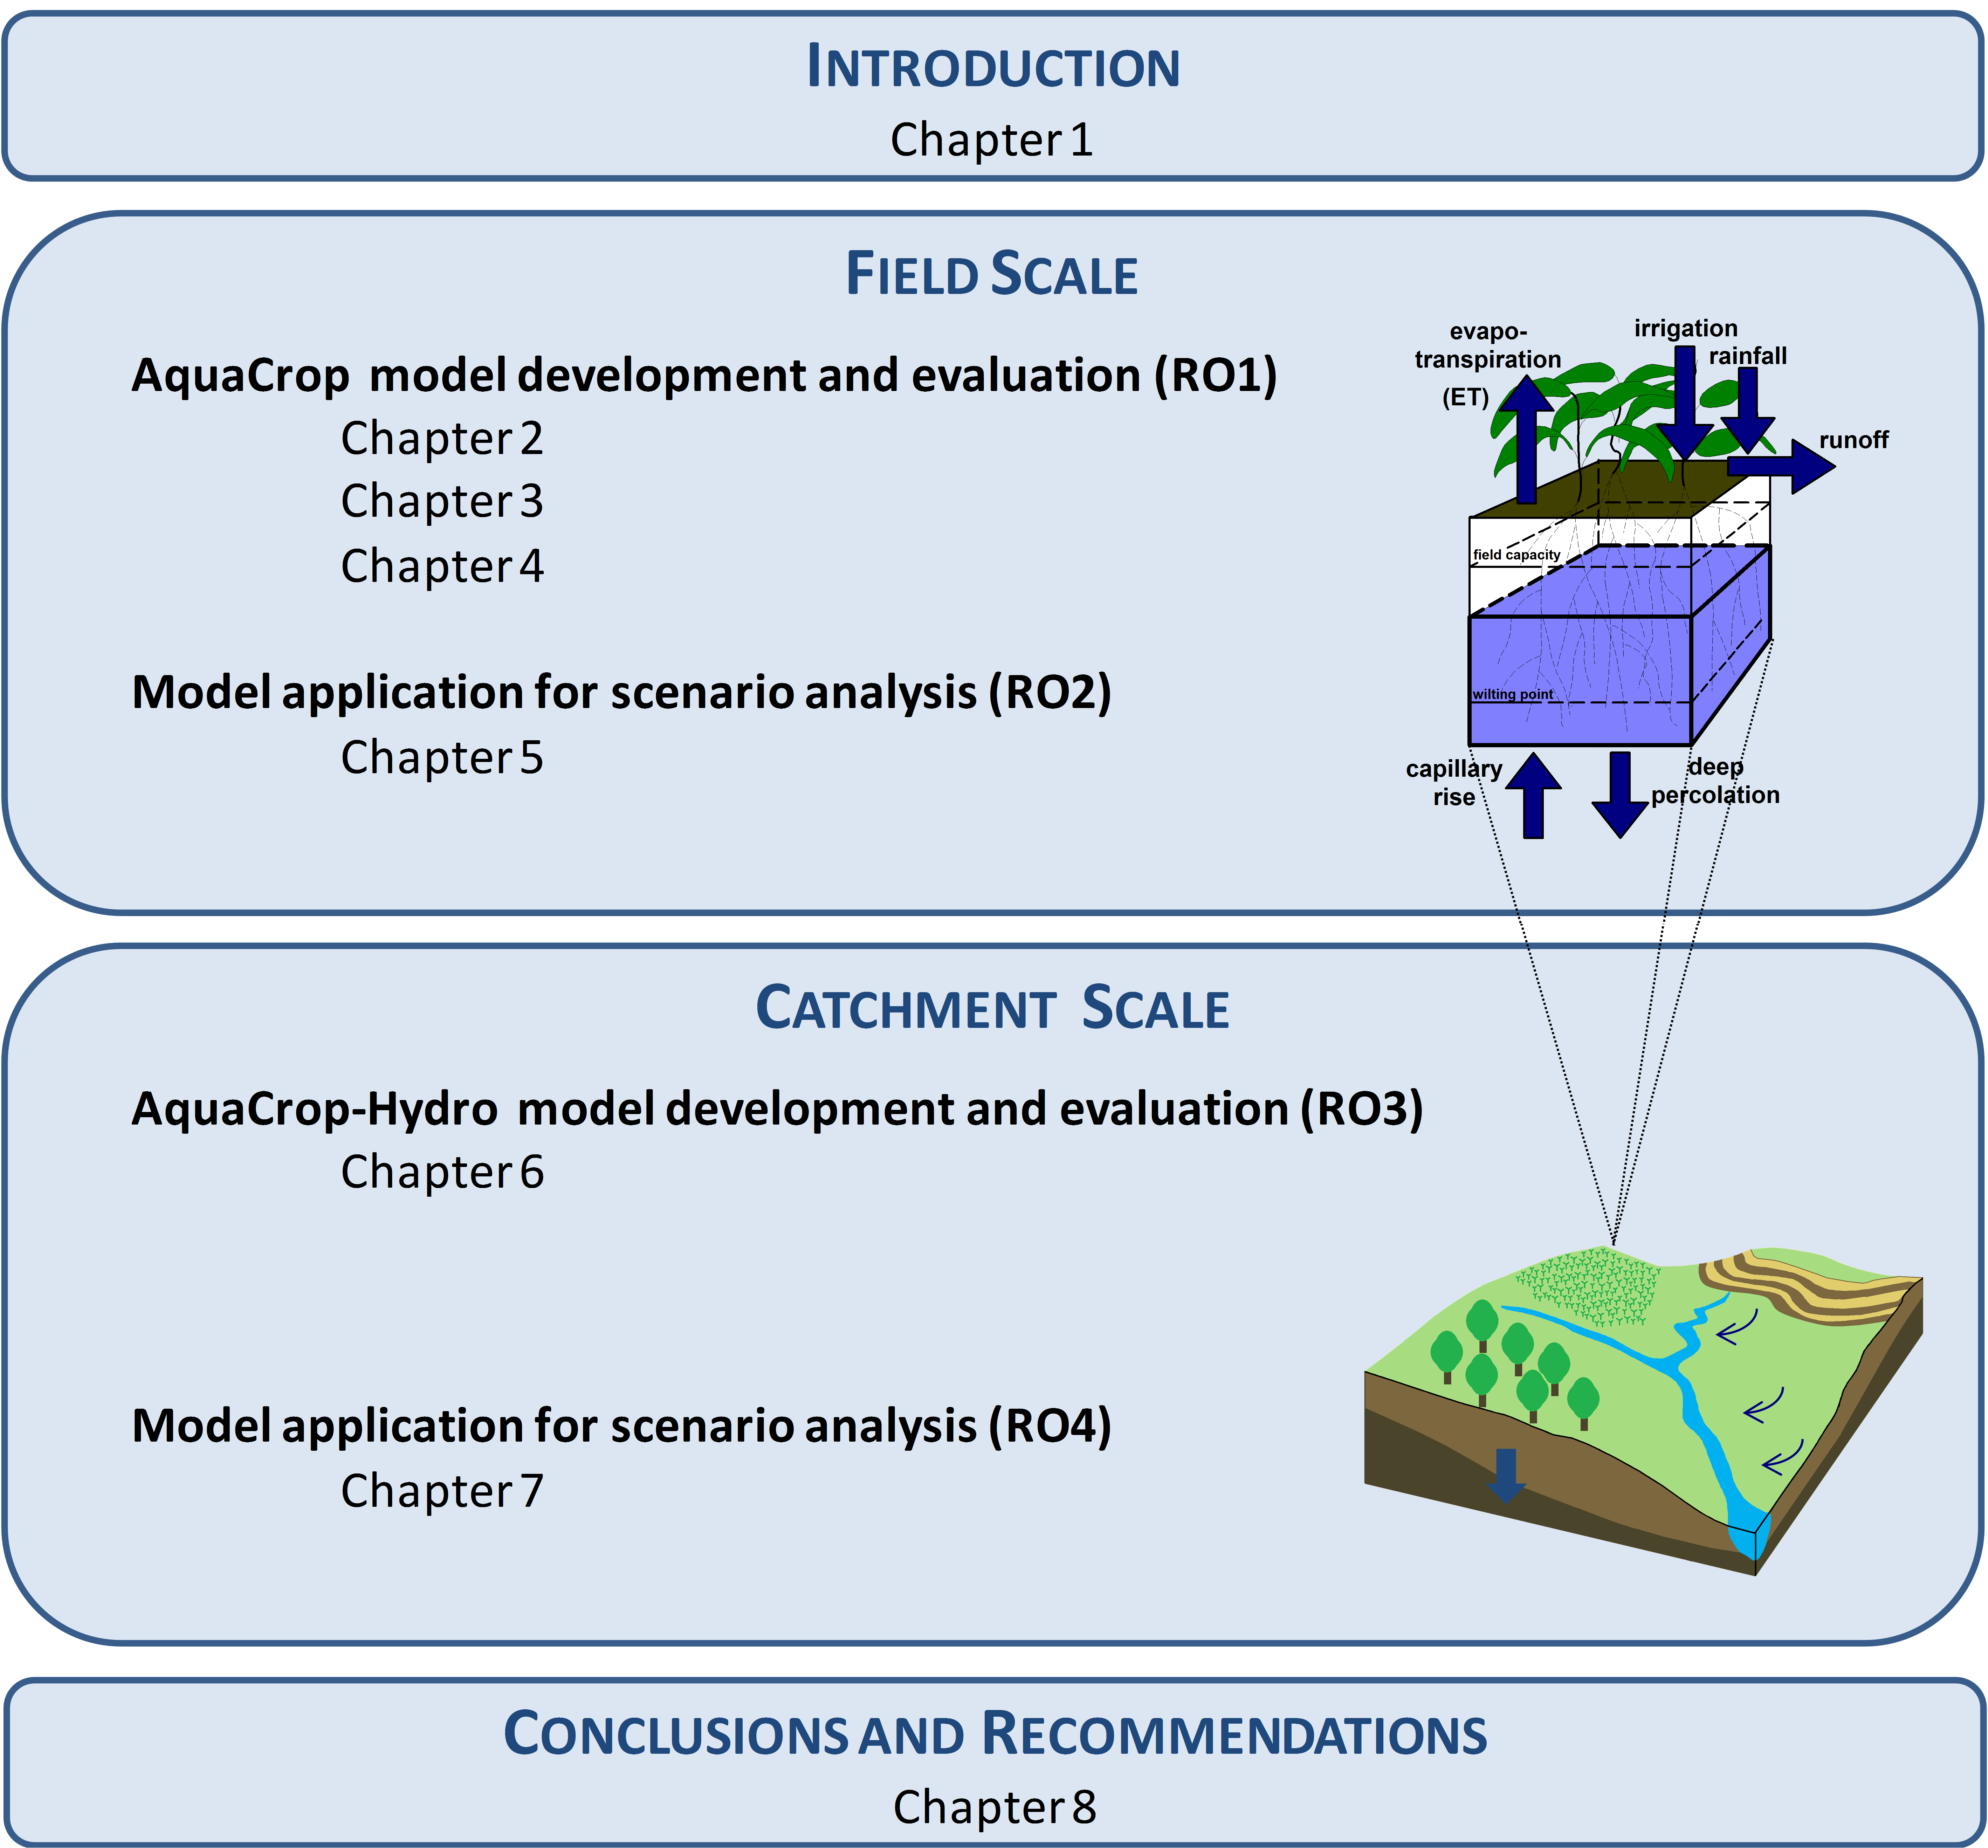
\includegraphics[width=\textwidth]{Structure_600dpi.png}
	\caption{Structure of the dissertation with indication of the research objectives (RO) and corresponding chapters.}
	\label{fig:ch1_Structure}
\end{figure}








			
\clearpage




%EXTRA TEXT

%With less than a quarter of the world's irrigated area located in developed countries, developing countries dominate irrigated agriculture. Furthermore, \textcite{fao2011} predicts a 17\% expansion of irrigated land between 2005 and 2050, almost exclusively located in developing countries. 
%This major increase in agricultural production needs to take place in a world where productive land is getting scarcer than ever, where several sectors and stakeholder struggle to get hold on the available natural resources and where one needs to deal with the burden of environmental pollution and the projected future climatic changes. Consequently, the necessary increase in crop water productivity must be achieved in a sustainable manner, making optimal use of the available resources and considering both the on and off-site consequences of agricultural management.

%Furthermore,\parencite{zwart2010} simulated that current water productivity levels of wheat vary between 0.2 kg of harvestable wheat per m3 of water consumed to 1.8 \si{kg/m^3}. This global water productivity range for wheat is in line with, although slightly lower than, the ranges reported by \parencite{zwart2004} and \textcite{liu2007}. Highest water productivity levels were found in temperate regions with high precipitation, while in rainfed systems with low precipitation rates values between 0.4 and 0.8 \si{kg/m^3} were more common \parencite{zwart2010}. Also \textcite{liu2007} reported that low water productivity levels are more often encountered for rainfed cropping systems than for irrigated cropping systems. 









%%%%%%%%%%%%%%%%%%%%%%%%%%%%%%%%%%%%%%%%%%%%%%%%%%
% Keep the following \cleardoublepage at the end of this file, 
% otherwise \includeonly includes empty pages.
\cleardoublepage

% vim: tw=70 nocindent expandtab foldmethod=marker foldmarker={{{}{,}{}}}
